\documentclass{beamer}
\usepackage[utf8]{inputenc}

\usetheme{Madrid}
\usecolortheme{default}
\usepackage{amsmath,amssymb,amsfonts,amsthm}
\usepackage{txfonts}
\usepackage{tkz-euclide}
\usepackage{listings}
\usepackage{adjustbox}
\usepackage{array}
\usepackage{tabularx}
\usepackage{gvv}
\usepackage{lmodern}
\usepackage{circuitikz}
\usepackage{tikz}
\usepackage{graphicx}
\usepackage{multicol}
\setbeamertemplate{page number in head/foot}[totalframenumber]

\usepackage{tcolorbox}
\tcbuselibrary{minted,breakable,xparse,skins}



\definecolor{bg}{gray}{0.95}
\DeclareTCBListing{mintedbox}{O{}m!O{}}{%
  breakable=true,
  listing engine=minted,
  listing only,
  minted language=#2,
  minted style=default,
  minted options={%
    linenos,
    gobble=0,
    breaklines=true,
    breakafter=,,
    fontsize=\small,
    numbersep=8pt,
    #1},
  boxsep=0pt,
  left skip=0pt,
  right skip=0pt,
  left=25pt,
  right=0pt,
  top=3pt,
  bottom=3pt,
  arc=5pt,
  leftrule=0pt,
  rightrule=0pt,
  bottomrule=2pt,

  colback=bg,
  colframe=orange!70,
  enhanced,
  overlay={%
    \begin{tcbclipinterior}
    \fill[orange!20!white] (frame.south west) rectangle ([xshift=20pt]frame.north west);
    \end{tcbclipinterior}},
  #3,
}
\lstset{
    language=C,
    basicstyle=\ttfamily\small,
    keywordstyle=\color{blue},
    stringstyle=\color{orange},
    commentstyle=\color{green!60!black},
    numbers=left,
    numberstyle=\tiny\color{gray},
    breaklines=true,
    showstringspaces=false,
}
%------------------------------------------------------------
%This block of code defines the information to appear in the
%Title page
\title %optional
{7.4.19}
\date{October  2025}
%\subtitle{A short story}

\author % (optional)
{BEERAM MADHURI - EE25BTECH11012}



\begin{document}


\frame{\titlepage}
\begin{frame}{Question}
Let $\mathbf{C}$ be the circle with centre $(0,0)$ and radius $3$ units. The equation of the locus of the mid points of the chords of the circle $\mathbf{C}$ that subtend an angle of $\frac{2\pi}{3}$ at its centre is

\begin{enumerate}
\begin{multicols}{4}
    \item $x^2 + y^2 = \frac{3}{2}$
    \item $x^2 + y^2 = 1$
    \item $x^2 + y^2 = \frac{27}{4}$
    \item $x^2 + y^2 = \frac{9}{4}$
\end{multicols}    
\end{enumerate}
\end{frame}
 
\begin{frame}{solution}
\frametitle{finding the locus:}
Given radius = $3$ units
\begin{align}
\vec{C} = \text{center} = \begin{pmatrix} 0 \\ 0 \end{pmatrix}
\end{align}

Let $\vec{A}$ and $\vec{B}$ be the end points of chord 
\begin{align}
\|\vec{A}\| = \|\vec{B}\| = 3 \\
\vec{A}^\top \vec{A} = 9 \\
\vec{B}^\top \vec{B} = 9 \\
\vec{A}^\top \vec{B} = \|\vec{A}\| \|\vec{B}\| \cos\theta = -\frac{9}{2} 
\end{align}
\end{frame}
\begin{frame}
Let $P$ be the midpoint of chords then, 
\begin{align}
\vec{P} = \frac{\vec{A + B}}{2} \\
\|\vec{P}\| = \frac{1}{2} \|\vec{A + B}\| \\
\vec{P^\top} \vec{P} = \frac{1}{4} (\vec{A+B})^\top (\vec{A+B}) \\
\vec{P^\top} \vec{P} = \frac{1}{4} (\vec{A^\top} \vec{A} + \vec{A^\top} \vec{B} + \vec{B^\top} \vec{A} + \vec{B^\top B})\\
\end{align}
\end{frame}
\begin{frame}
Substituting the values:
\begin{align}
\quad = \frac{1}{4} \left(9 - \frac{9}{2} - \frac{9}{2} + 9\right) = \frac{9}{4}
\end{align}
Hence, $\vec{P^\top} \vec{P}$ =${9}/{4}$\\
option {D} is correct.
\end{frame}


\begin{frame}[fragile]
    \frametitle{Python Code}
    \begin{lstlisting}
import numpy as np
import matplotlib.pyplot as plt
from matplotlib.patches import Arc

# --- 1. Setup the figure and axis ---
fig, ax = plt.subplots(figsize=(8, 8))
ax.set_aspect('equal', adjustable='box')
ax.grid(True, linestyle='--', alpha=0.6)
ax.axhline(0, color='black', linewidth=0.5)
ax.axvline(0, color='black', linewidth=0.5)
\end{lstlisting}
\end{frame}

\begin{frame}[fragile]
\frametitle{python Code}
\begin{lstlisting}
# --- 2. Define and plot the original circle (C) ---
r_C = 3
theta = np.linspace(0, 2 * np.pi, 200)
x_C = r_C * np.cos(theta)
y_C = r_C * np.sin(theta)
ax.plot(x_C, y_C, 'b-', label=r'Original Circle C: $x^2 + y^2 = 9$')
\end{lstlisting}
\end{frame}

\begin{frame}[fragile]
\frametitle{python Code}
\begin{lstlisting}
# --- 3. Define and plot the locus of midpoints ---
# The distance of the midpoint from the center is r_C * cos((2pi/3)/2) = 3 * cos(pi/3) = 1.5
r_locus = 1.5
x_locus = r_locus * np.cos(theta)
y_locus = r_locus * np.sin(theta)
ax.plot(x_locus, y_locus, 'r--', label=r'Locus of Midpoints: $x^2 + y^2 = \frac{9}{4}$')

# --- 4. Draw an example chord and radii to illustrate ---
# Angle of the radius to the chord midpoint
angle_midpoint = np.pi / 4
\end{lstlisting}
\end{frame}

\begin{frame}[fragile]
\frametitle{python Code}
\begin{lstlisting}
# Center
O = (0, 0)
# Midpoint P
P = (r_locus * np.cos(angle_midpoint), r_locus * np.sin(angle_midpoint))
# Endpoints of the chord (A and B)
angle_subtended_half = np.pi / 3  # Half of 2pi/3
A = (r_C * np.cos(angle_midpoint + angle_subtended_half), r_C * np.sin(angle_midpoint + angle_subtended_half))
B = (r_C * np.cos(angle_midpoint - angle_subtended_half), r_C * np.sin(angle_midpoint - angle_subtended_half))
\end{lstlisting}
\end{frame}

\begin{frame}[fragile]
\frametitle{python Code}
\begin{lstlisting}
# Plot the illustrative elements
ax.plot([A[0], B[0]], [A[1], B[1]], 'g-', label=r'Example Chord subtending $\frac{2\pi}{3}$') # Chord AB
ax.plot([O[0], A[0]], [O[1], A[1]], 'k:', alpha=0.8) # Radius OA
ax.plot([O[0], B[0]], [O[1], B[1]], 'k:', alpha=0.8) # Radius OB
ax.plot([O[0], P[0]], [O[1], P[1]], 'm-', alpha=0.8) # Line to midpoint OP
# Plot and label the points
ax.plot(O[0], O[1], 'ko')
ax.text(O[0] - 0.2, O[1] - 0.2, 'O', fontsize=12)
ax.plot(P[0], P[1], 'mo')
ax.text(P[0] + 0.1, P[1] + 0.1, 'P (midpoint)', fontsize=12, color='m')
\end{lstlisting}
\end{frame}

\begin{frame}[fragile]
\frametitle{python Code}
\begin{lstlisting}
# Add angle annotation
angle_rad = 2 * np.pi / 3
arc = Arc(O, 2, 2, angle=0,
          theta1=np.degrees(angle_midpoint - angle_subtended_half),
          theta2=np.degrees(angle_midpoint + angle_subtended_half),
          color='purple', lw=1.5, linestyle='-')
ax.add_patch(arc)
angle_text_pos = (0.8 * np.cos(angle_midpoint), 0.8 * np.sin(angle_midpoint))
ax.text(angle_text_pos[0], angle_text_pos[1], r'$\frac{2\pi}{3}$', fontsize=14, color='purple', ha='center', va='center')
\end{lstlisting}
\end{frame}

\begin{frame}[fragile]
\frametitle{python Code}
\begin{lstlisting}

# --- 5. Finalize and show the plot ---
ax.set_title('Locus of the Midpoints of Chords', fontsize=16)
ax.set_xlabel('x-axis')
ax.set_ylabel('y-axis')
ax.legend()
plt.xlim(-3.5, 3.5)
plt.ylim(-3.5, 3.5)
plt.show()
\end{lstlisting}
\end{frame}

\begin{frame}[fragile]
\frametitle{C Code}
\begin{lstlisting}
 #include <stdio.h>
#include <math.h>

// Define PI if it's not available in math.h (M_PI is common but not standard)
#ifndef M_PI
#define M_PI 3.14159265358979323846
#endif
\end{lstlisting}
\end{frame}

\begin{frame}[fragile]
\frametitle{C Code}
\begin{lstlisting}
int main() {
    // --- Given Parameters ---
    // Radius of the main circle C
    double radius = 3.0; 
    // Angle subtended by the chords at the center in radians
    double angle_rad = (2.0 * M_PI) / 3.0;
    // The locus of the midpoints is another circle. Its radius (let's call it r_locus)
    // is found using the formula: r_locus = radius * cos(angle / 2).
\end{lstlisting}
\end{frame}

\begin{frame}[fragile]
\frametitle{C Code}
\begin{lstlisting}    
    // 1. Find half the angle
    double half_angle = angle_rad / 2.0;
    // 2. Calculate the radius of the locus circle
    double locus_radius = radius * cos(half_angle);
    // 3. The equation of the locus is x^2 + y^2 = (locus_radius)^2.
    //    We need to find the value of the radius squared.
    double locus_radius_squared = pow(locus_radius, 2);
\end{lstlisting}
\end{frame}

\begin{frame}[fragile]
\frametitle{C Code}
\begin{lstlisting}
    // --- Output ---
    printf("Problem: Find the locus of the midpoints of chords of the circle x^2 + y^2 = %.0f\n", pow(radius, 2));
    printf("where the chords subtend an angle of 2*pi/3 at the center.\n\n");
    
    printf("--- Calculation Results ---\n");
    printf("Radius of the locus circle: %.2f\n", locus_radius);
\end{lstlisting}
\end{frame}

\begin{frame}[fragile]
\frametitle{C Code}
\begin{lstlisting}
    printf("Radius of the locus circle squared: %.2f\n\n", locus_radius_squared);

    printf("The final equation of the locus is: x^2 + y^2 = %.2f\n", locus_radius_squared);
    printf("This corresponds to option (d): x^2 + y^2 = 9/4\n");

    return 0;
}
\end{lstlisting}
\end{frame}

\begin{frame}[fragile]
\frametitle{Python and C Code}
\begin{lstlisting}
from ctypes import c_double
import math

# Define M_PI if not available
M_PI = math.pi

# --- Given Parameters ---
# Radius of the main circle C
radius = c_double(3.0)
\end{lstlisting}
\end{frame}

\begin{frame}[fragile]
\frametitle{Python and C Code}
\begin{lstlisting}
# Angle subtended by the chords at the center in radians
angle_rad = c_double((2.0 * M_PI) / 3.0)

# --- Calculation ---
# 1. Find half the angle
half_angle = c_double(angle_rad.value / 2.0)

# 2. Calculate the radius of the locus circle
locus_radius = c_double(radius.value * math.cos(half_angle.value))
\end{lstlisting}
\end{frame}

\begin{frame}[fragile]
\frametitle{Python and C Code}
\begin{lstlisting}
# 3. Radius squared
locus_radius_squared = c_double(math.pow(locus_radius.value, 2))

# --- Output ---
print(f"Problem: Find the locus of the midpoints of chords of the circle x^2 + y^2 = {math.pow(radius.value, 2):.0f}")
print("where the chords subtend an angle of 2*pi/3 at the center.\n")
\end{lstlisting}
\end{frame}

\begin{frame}[fragile]
\frametitle{Python and C Code}
\begin{lstlisting}
print("--- Calculation Results ---")
print(f"Radius of the locus circle: {locus_radius.value:.2f}")
print(f"Radius of the locus circle squared: {locus_radius_squared.value:.2f}\n")
print(f"The final equation of the locus is: x^2 + y^2 = {locus_radius_squared.value:.2f}")
print("This corresponds to option (d): x^2 + y^2 = 9/4")

\end{lstlisting}
\end{frame}

\begin{figure}[H]
    \centering
    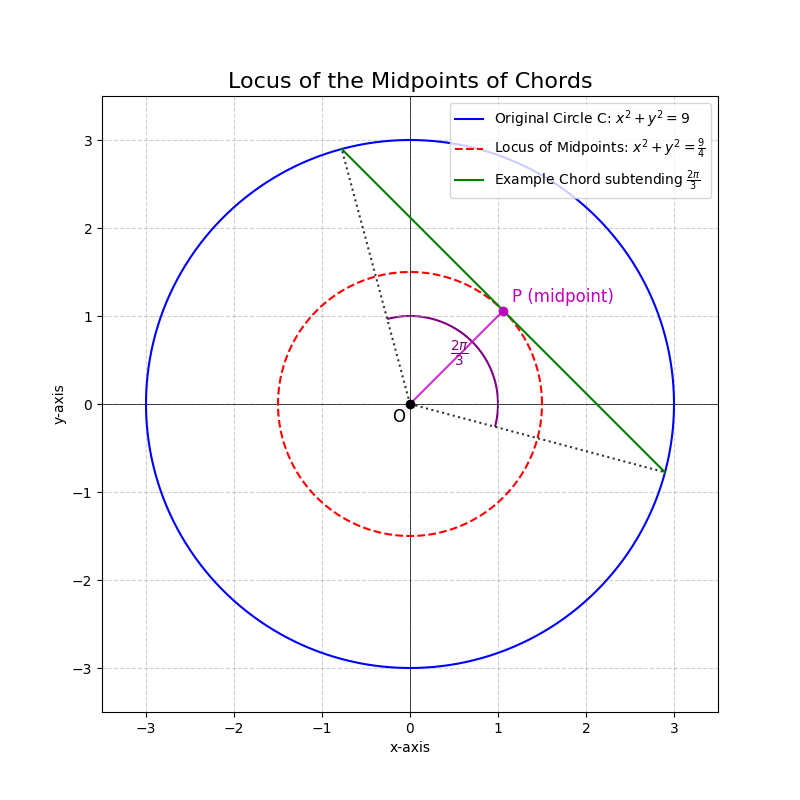
\includegraphics[width=0.7\columnwidth]{graph14.png}
    \caption{Plot}
    \label{fig:placeholder}
\end{figure}


\end{document}